\documentclass[tikz]{standalone}
\usepackage{pgfplots}
\pgfplotsset{compat=1.15}
\usepackage{mathrsfs}
\usetikzlibrary{arrows,calc}
\usepackage{tkz-euclide}

\pagestyle{empty}

\definecolor{AngleClr}{rgb}{0,0.39215686274509803,0}
\definecolor{ShapeClr}{rgb}{0.6,0.2,0}

\begin{document}

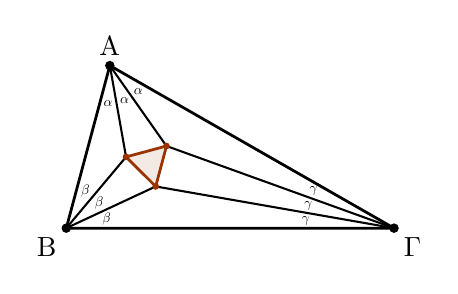
\begin{tikzpicture}[scale=.75]
\tkzSetUpLine[line width=1pt,color=black]
\tkzSetUpPoint[fill=black]

\tkzDefPoints{0/0/C,5.55/0/B}
\tkzDefPoint(75:2.85){A}

\tkzFindAngle(C,A,B) \tkzGetAngle{anglea}
\tkzDefPointBy[rotation=center A angle 1*\anglea/3](C) \tkzGetPoint{TA1}
\tkzDefPointBy[rotation=center A angle 2*\anglea/3](C) \tkzGetPoint{TA2}
\tkzFindAngle(A,B,C) \tkzGetAngle{angleb}
\tkzDefPointBy[rotation=center B angle 1*\angleb/3](A) \tkzGetPoint{TB1}
\tkzDefPointBy[rotation=center B angle 2*\angleb/3](A) \tkzGetPoint{TB2}
\tkzFindAngle(B,C,A) \tkzGetAngle{anglec}
\tkzDefPointBy[rotation=center C angle 1*\anglec/3](B) \tkzGetPoint{TC1}
\tkzDefPointBy[rotation=center C angle 2*\anglec/3](B) \tkzGetPoint{TC2}
% \tkzInterLL(A,TA1)(B,TB2) \tkzGetPoint{U1}
\tkzInterLL(A,TA2)(B,TB1) \tkzGetPoint{V1}
% \tkzInterLL(B,TB1)(C,TC2) \tkzGetPoint{U2}
\tkzInterLL(B,TB2)(C,TC1) \tkzGetPoint{V2}
% \tkzInterLL(C,TC1)(A,TA2) \tkzGetPoint{U3}
\tkzInterLL(C,TC2)(A,TA1) \tkzGetPoint{V3}
%  U1,U2,U3)
% \tkzDrawLines[add=2 and 2,very thin,dashed](A,TA1 B,TB1 C,TC1 A,TA2 B,TB2 C,TC2)
% \tkzDrawPoints(U1,U2,U3,V1,V2,V3)

\tkzFillPolygon[fill=white](A,B,C)
\tkzFillPolygon[fill=ShapeClr,fill opacity=0.1](V1,V2,V3)

\tkzDrawSegments[line width=0.75pt](A,V1 A,V3 B,V1 B,V2 C,V3 C,V2)
\tkzDrawPolygons[color=ShapeClr](V1,V2,V3)
\tkzDrawPolygons[color=black](A,B,C)

\tkzDrawPoints[color=ShapeClr,size=2](V1,V2,V3)
\tkzDrawPoints[size=3](A,B,C)
\tkzLabelPoint[above](A){$\rm A$}
\tkzLabelPoint[below left](C){$\rm B$}
\tkzLabelPoint[below right](B){$\rm \Gamma$}

\tkzLabelAngles[pos=0.65](V1,A,B){\scalebox{0.5}{$\alpha$}}
\tkzLabelAngles[pos=0.65](V3,A,V1){\scalebox{0.5}{$\alpha$}}
\tkzLabelAngles[pos=0.65](C,A,V3){\scalebox{0.5}{$\alpha$}}
\tkzLabelAngles[pos=1.5](A,B,V1 V1,B,V2 V2,B,C){\scalebox{0.5}{$\gamma$}}

\tkzLabelAngles[pos=0.7](B,C,V2 V2,C,V3 V3,C,A){\scalebox{0.5}{$\beta$}}

\end{tikzpicture}
\end{document}
